Das Wort \texttt{1+2+3+4+5} hat zwei mögliche Parse-Trees mit der 
untenstehenden Grammatik.
Ergänzen Sie die Variablen und finden Sie die die Unterteilungen des
Wortes gemäss dem Beweis des Pumping-Lemma.
\begin{center}
\def\dx{0.4}
\def\dy{0.5}
\def\punkt#1#2{
	({((#1)-0.5*(#2))*\dx},{(-(#2))*\dy})
}
\def\gabel#1#2#3#4{
	\draw \punkt{#1}{#2} -- \punkt{#1}{#2+#3};
	\draw \punkt{#1}{#2} -- \punkt{#1+#4}{#2+#4};
}
\def\wort{
	\node at \punkt{0.25}{8.5} {\texttt{1}\strut};
	\node at \punkt{1.25}{8.5} {\texttt{+}\strut};
	\node at \punkt{2.25}{8.5} {\texttt{2}\strut};
	\node at \punkt{3.25}{8.5} {\texttt{+}\strut};
	\node at \punkt{4.25}{8.5} {\texttt{3}\strut};
	\node at \punkt{5.25}{8.5} {\texttt{+}\strut};
	\node at \punkt{6.25}{8.5} {\texttt{4}\strut};
	\node at \punkt{7.25}{8.5} {\texttt{+}\strut};
	\node at \punkt{8.25}{8.5} {\texttt{5}\strut};
}
\begin{tikzpicture}[>=latex,thick]
\begin{scope}[xshift=-0.3*\textwidth]
\node at \punkt{3.5}{3.5} {$\begin{aligned}
A & \to AB \\
  & \to \texttt{0}\mid\texttt{1}\mid \ldots\mid\texttt{9} \\
B & \to PA \\
P & \to \texttt{+} 
\end{aligned}$};
\end{scope}
\begin{scope}
\gabel{0}{0}{4}{5}
	\gabel{0}{4}{2}{3}
		\gabel{0}{6}{2}{1}
			\gabel{1}{7}{1}{1}
		\gabel{3}{7}{1}{1}
	\gabel{5}{5}{3}{1}
		\gabel{6}{6}{2}{1}
			\gabel{7}{7}{1}{1}
\begin{scope}[yshift=-0.1cm]
\wort
\end{scope}
\end{scope}
\begin{scope}[xshift=0.3*\textwidth]
\gabel{0}{0}{2}{7}
	\gabel{0}{2}{2}{5}
		\gabel{0}{4}{4}{1}
			\gabel{1}{5}{3}{1}
				\gabel{2}{6}{2}{1}
					\gabel{3}{7}{1}{1}
		\gabel{5}{7}{1}{1}
	\gabel{7}{7}{1}{1}
\begin{scope}[yshift=-0.1cm]
\wort
\end{scope}
\end{scope}
\end{tikzpicture}
\end{center}

\begin{loesung}
Die Grammatik hat zwar nicht ganz Chomsky-Normalform, weil die Startvariable
auch auf der rechten Seite vorkommt, für die Zwecke des Pumping Lemmas
reicht diese Form jedoch.
\begin{center}
\def\dx{0.6}
\def\dy{0.8}
\def\punkt#1#2{
	({((#1)-0.5*(#2))*\dx},{(-(#2))*\dy})
}
\def\terminal#1#2#3{
	\fill[color=white] \punkt{#1}{#2} circle[radius=0.15];
	\node at \punkt{#1}{#2} {$#3\mathstrut$};
}
\def\gabel#1#2#3#4#5{
	\draw \punkt{#1}{#2} -- \punkt{#1}{#2+#3};
	\draw \punkt{#1}{#2} -- \punkt{#1+#4}{#2+#4};
	\fill[color=white] \punkt{#1}{#2} circle[radius=0.15];
	\node at \punkt{#1}{#2} {$#5\mathstrut$};
}
\def\wort{
	\node at \punkt{0.25}{8.5} {\texttt{1}\strut};
	\node at \punkt{1.25}{8.5} {\texttt{+}\strut};
	\node at \punkt{2.25}{8.5} {\texttt{2}\strut};
	\node at \punkt{3.25}{8.5} {\texttt{+}\strut};
	\node at \punkt{4.25}{8.5} {\texttt{3}\strut};
	\node at \punkt{5.25}{8.5} {\texttt{+}\strut};
	\node at \punkt{6.25}{8.5} {\texttt{4}\strut};
	\node at \punkt{7.25}{8.5} {\texttt{+}\strut};
	\node at \punkt{8.25}{8.5} {\texttt{5}\strut};
}
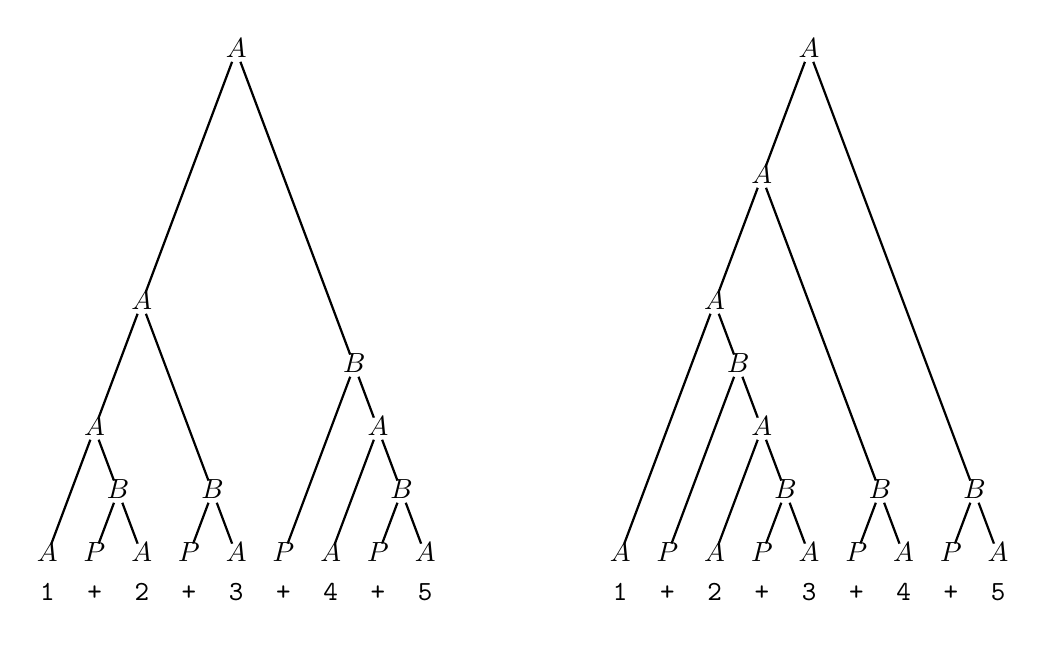
\begin{tikzpicture}[>=latex,thick]

\begin{scope}[xshift=-0.3*\textwidth]
	\gabel{0}{0}{4}{5}{A}
		\gabel{0}{4}{2}{3}{A}
			\gabel{0}{6}{2}{1}{A}
				\gabel{1}{7}{1}{1}{B}
			\gabel{3}{7}{1}{1}{B}
		\gabel{5}{5}{3}{1}{B}
			\gabel{6}{6}{2}{1}{A}
				\gabel{7}{7}{1}{1}{B}
	\terminal{0}{8}{A}
	\terminal{1}{8}{P}
	\terminal{2}{8}{A}
	\terminal{3}{8}{P}
	\terminal{4}{8}{A}
	\terminal{5}{8}{P}
	\terminal{6}{8}{A}
	\terminal{7}{8}{P}
	\terminal{8}{8}{A}
	\begin{scope}[yshift=-0.1cm]
		\wort
	\end{scope}
\end{scope}

\begin{scope}[xshift=0.3*\textwidth]
	\gabel{0}{0}{2}{7}{A}
		\gabel{0}{2}{2}{5}{A}
			\gabel{0}{4}{4}{1}{A}
				\gabel{1}{5}{3}{1}{B}
					\gabel{2}{6}{2}{1}{A}
						\gabel{3}{7}{1}{1}{B}
			\gabel{5}{7}{1}{1}{B}
		\gabel{7}{7}{1}{1}{B}
	\terminal{0}{8}{A}
	\terminal{1}{8}{P}
	\terminal{2}{8}{A}
	\terminal{3}{8}{P}
	\terminal{4}{8}{A}
	\terminal{5}{8}{P}
	\terminal{6}{8}{A}
	\terminal{7}{8}{P}
	\terminal{8}{8}{A}
	\begin{scope}[yshift=-0.1cm]
		\wort
	\end{scope}
\end{scope}

\end{tikzpicture}
\end{center}
\end{loesung}



